\section{System Architecture}
\label{sec:system-overview:architecture}

The proposed interlocking system is structured into three interconnected layers, each with distinct responsibilities but designed to operate cohesively as part of a unified framework (illustrated in Figure~\ref{fig:top-level-view}). At the top sits the frontend operator interface, developed using Qt’s graphical framework. This interface provides dispatchers with a real-time, interactive view of the station layout, enabling them to issue route commands, monitor signal aspects and track occupancy, and receive immediate feedback on system status. Beyond its monitoring role, the frontend is designed with usability in mind, ensuring that complex interlocking operations can be executed quickly and reliably under the pressure of live railway operations.

\begin{figure}[t]
    \centering

    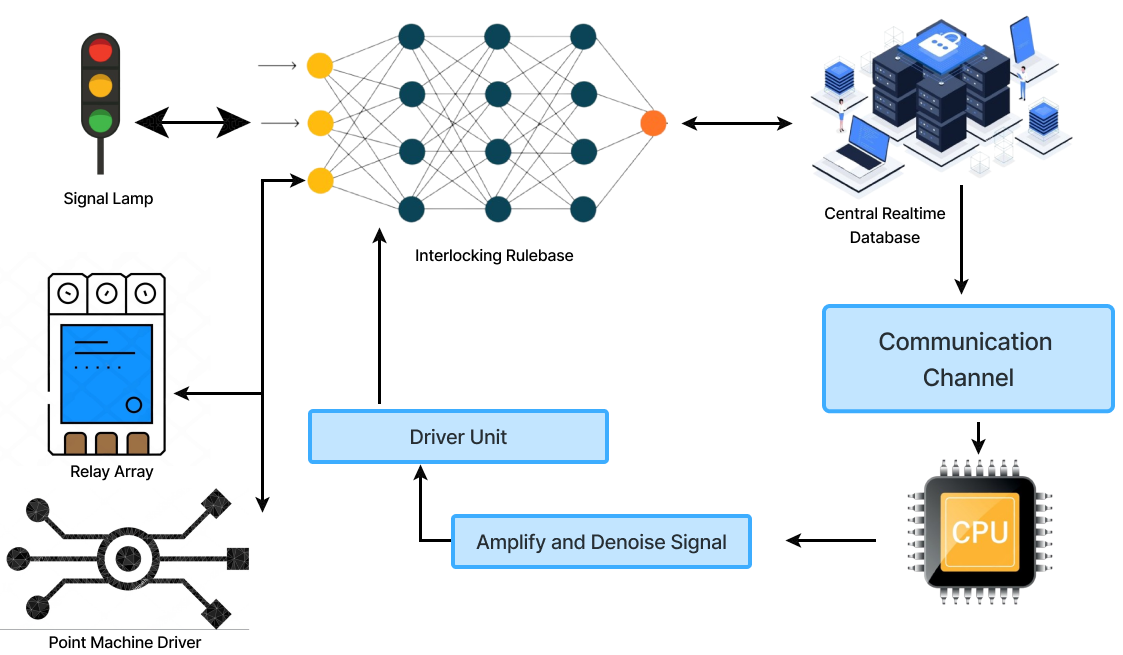
\includegraphics[width=0.85\textwidth]{images/architecture-diagrams/high-level-view.png}

    \floatcap{Top Level System Architecture}{This diagram illustrates how the major blocks of the system connected to each other.}
    
    \label{fig:top-level-view}
\end{figure}


Beneath the interface lies the backend logic engine, implemented in Qt C++. This core layer functions as the decision-making hub, executing interlocking rules, validating route requests, and coordinating the flow of events across the system. It encapsulates the safety logic, ensuring that all route settings and signal clearances conform to the constraints defined by interlocking principles. The engine is built with modularity in mind, allowing logic to be extended or reconfigured as operational needs evolve. Its reliance on Qt’s event-driven model, particularly signals and slots, enables asynchronous communication that preserves determinism while supporting real-time responsiveness.

At the foundation is the database layer, implemented on PostgreSQL. This layer manages both static configuration data, such as station topology and route definitions, and dynamic state data, including signal aspects, point machine positions, and track circuit occupancy. By consolidating both structural and operational information in a relational model, the database serves as the system’s single source of truth, enabling traceability, rollback functionality, and forensic analysis of past events. Its integration with database triggers and stored procedures also enhances fault tolerance by allowing critical validations to be enforced at the persistence level, creating a multi-layer safety net across the architecture.

Communication between these layers is facilitated through service interfaces, structured queries, and event emitters, following a loosely coupled service-based design. This architecture not only simplifies system extension and testing but also ensures resilience by isolating failures within individual layers. The result is a scalable and transparent interlocking framework that balances real-time performance with maintainability, making it adaptable for both simulation environments and future hardware-in-the-loop deployments.